\chapter{Preprocessing}

Quella che sarà descritta in questa sezione è la fase più impegnativa e delicata. 

\section{Preparazione dell'Ambiente di Lavoro}

	\subsection{Ottenere gli strumenti necessari}

		\begin{lstlisting}[language=bash,caption={installazione di MongoDB}]
			sudo pacman -S mongodb mongodb-tools
		\end{lstlisting}

		\begin{lstlisting}[language=bash,caption={installazione di pymongo}]
			pip install pymongo
		\end{lstlisting}

	\subsection{Inizializzazione di un server MongoDB}

		\begin{lstlisting}[language=bash,caption={script di lancio di un server MongoDB}, numbers=left, stepnumber=1]
			#!/bin/zsh
			sudo killall mongod
			yes | rm -rf /mnt/ramdisk/db
			mkdir db /mnt/ramdisk/db
			mongod --dbpath=/mnt/ramdisk/db
		\end{lstlisting}

	\subsection{Importazione dei Dati Grezzi}

	\begin{center}
		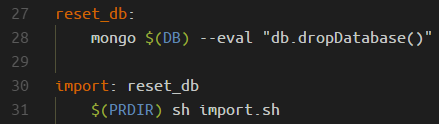
\includegraphics[scale=0.7]{img/import.png}
	\end{center}

	\lstinputlisting[language=bash,caption={script per importare i dati grezzi in MongoDB}, numbers=left, stepnumber=1]{../prepr/import.sh}

\section{Valutazioni degli Insegnamenti aggregate per Anno Accademico}

\section{Join dei due insiemi di dati con attributi continui}

\section{Join dei due insiemi di dati con attributi discreti}

\section{Sequenze ordinate di esami superati}

\section{Estrazione dei data set preprocessati}

	\begin{center}
		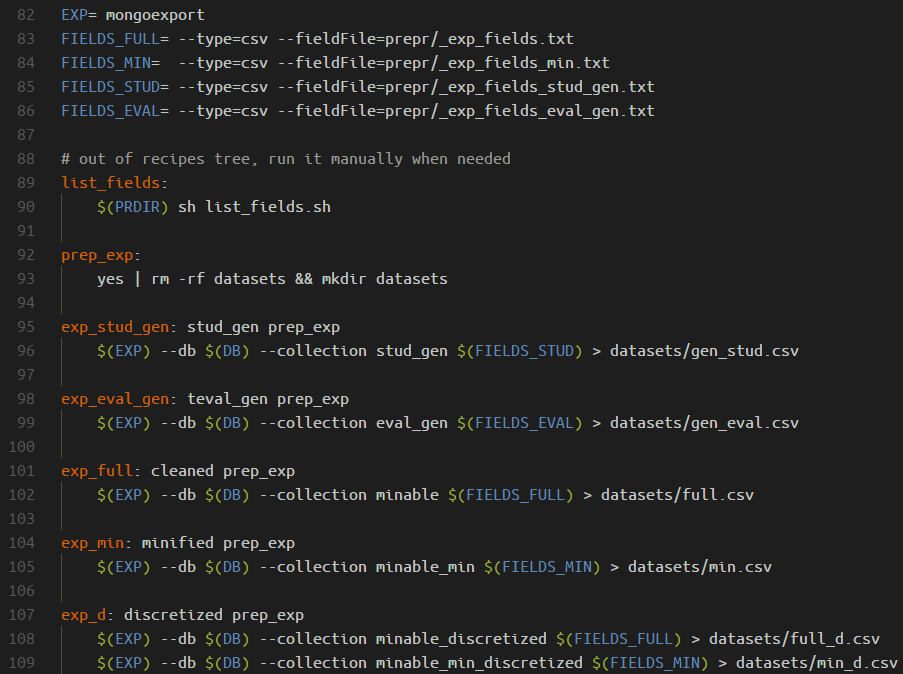
\includegraphics[scale=0.7]{img/export.png}
	\end{center}

	\lstinputlisting[language=bash,caption={script di shell per ottenere una lista degli attributi dei documenti in una collezione}, numbers=left, stepnumber=1]{../prepr/list_fields.sh}

	\lstdefinelanguage{JavaScript}{
  		keywords={break, case, catch, continue, debugger, default, delete, do, else, finally, for, function, if, in, instanceof, new, return, switch, this, throw, try, typeof, var, void, while, with},
 		morecomment=[l]{//},
  		morecomment=[s]{/*}{*/},
  		morestring=[b]',
  		morestring=[b]",
  		sensitive=true
	}

	\lstinputlisting[language=JavaScript,caption={script della shell di MongoDB per ottenere la lista degli attributi dei documenti in una collezione}, numbers=left, stepnumber=1]{../prepr/list_attr.mongosh}
